\documentclass[a4paper, openany]{memoir}

\usepackage[utf8]{inputenc}
\usepackage[T1]{fontenc} 
\usepackage[english]{babel}
\usepackage{fancyhdr}
\usepackage{float}
\usepackage{amsmath, amsthm, amssymb}
\usepackage{enumitem}
\usepackage[bookmarksopen=true,bookmarksopenlevel=2]{hyperref}
\usepackage{tikz}
\usepackage{pgfplots}
\usepackage{indentfirst}
\usepackage{pgfplots}
\usepackage{listings}

\pagestyle{fancy}
\fancyhf{}
\fancyhead[LE]{\leftmark}
\fancyhead[RO]{\rightmark}
\fancyhead[RE, LO]{Database Systems}
\fancyfoot[LE, RO]{\thepage}
\fancyfoot[RE, LO]{Pete Gautam}

\renewcommand{\headrulewidth}{1.5pt}

\theoremstyle{definition}
\newtheorem{definition}{Definition}[section]

\theoremstyle{plain}
\newtheorem{theorem}[definition]{Theorem}
\newtheorem{lemma}[definition]{Lemma}
\newtheorem{proposition}[definition]{Proposition}
\newtheorem{corollary}[definition]{Corollary}
\newtheorem{example}[definition]{Example}

\chapterstyle{thatcher}
\setcounter{chapter}{3}
\pgfplotsset{compat=newest}

\newcommand{\tuplesorted}[0]{
    \draw (0, 0) -- (1.5, 0)
    -- (1.5, -4)
    -- (0, -4)
    -- cycle;

    \foreach \x/\y[count=\i] in {1/2, 2/3, 2/5, 3/8, 5/9, 5/11, 5/12, 6/13} {
        \draw (0.75, -\i*0.5) -- (0.75, -\i*0.5 + 0.5);
        \draw (0, -\i*0.5) -- (1.5, -\i*0.5);
        \filldraw[blue!30, opacity=0.3] (0.75, -\i*0.5) -- (1.5, -\i*0.5)
            -- (1.5, -\i*0.5 + 0.5)
            -- (0.75, -\i*0.5 + 0.5)
            -- cycle;
        \filldraw[red!30, opacity=0.3] (0.75, -\i*0.5) -- (0, -\i*0.5)
            -- (0, -\i*0.5 + 0.5)
            -- (0.75, -\i*0.5 + 0.5)
            -- cycle;
        \node at (0.375, -\i*0.5 + 0.25) {\texttt{\x}};
        \node at (1.125, -\i*0.5 + 0.25) {\texttt{\y}};
    }

    \draw (4.5, 0) -- (5.25, 0)
        -- (5.25, -3)
        -- (4.5, -3)
        -- cycle;
        
    \foreach \i in {1, 2, ..., 6} {
        \draw (4.5, -\i * 0.5) -- (5.25, -\i * 0.5);
        \filldraw[red!30, opacity=0.3] (4.5, -\i*0.5) -- (5.25, -\i*0.5)
            -- (5.25, -\i*0.5 + 0.5)
            -- (4.5, -\i*0.5 + 0.5)
            -- cycle;
        \node at (4.875, -\i*0.5 + 0.25) {\texttt{\i}};
    }
}

\definecolor{codegreen}{rgb}{0,0.6,0}
\definecolor{codegray}{rgb}{0.5,0.5,0.5}
\definecolor{codepurple}{rgb}{0.58,0,0.82}
\definecolor{backcolour}{rgb}{0.95,0.95,0.92}

\lstdefinestyle{thestyle}{
    backgroundcolor=\color{backcolour},
    basicstyle=\ttfamily\footnotesize,
    keywordstyle=\color{red!80}\bfseries,
    ndkeywordstyle=\color{blue!80}\bfseries,
    identifierstyle=\color{black},
    commentstyle=\color{codegreen},
    stringstyle=\color{codepurple},
    breakatwhitespace=false,
    breaklines=true,
    captionpos=b,
    keepspaces=true,
    % numberstyle=\tiny\color{codegray},
    % numbers=left,
    % numbersep=2pt,
    showspaces=false,
    showstringspaces=false,
    showtabs=false,          
    tabsize=2
}

\lstset{style=thestyle}
\chapterstyle{thatcher}
\setcounter{chapter}{2}

\begin{document}
\chapter{Query Optimisation}
\section{Query Processing}
Almost all SQL queries involve sorting of tuples with respect to sorting requests defined by the user, e.g.
\begin{itemize}
    \item \texttt{CREATE PRIMARY INDEX ON EMPLOYEE(SSN)} means that we sort by \texttt{SSN}
    \item \texttt{ORDER BY Name} means that we sort by \texttt{Name}
    \item \texttt{SELECT DISTINCT Salary} means that we sort by \texttt{Salary} to create clusters, and then identify the distinct values
    \item \texttt{SELECT DNO, COUNT(*) FROM EMPLOYEE GROUP BY DNO} means that we sort by \texttt{DNO} to create clusters, and then count the number of values per cluster.
\end{itemize}
Normally, we cannot store the entire relation into memory for sorting the records. So, to sort the tuples, we use external sorting algorithm.

\subsection{External Sorting}
The external sorting algorithm is a divide and conquer algorithm. We first divide a file of $b$ blocks into $L$ smaller sub-files (so each sub-file has $b/L$ blocks). We require each of the sub-file to fit in memory. We load each small sub-file into memory and sort them (e.g. using quicksort) and then write it back to the disk. At the end of this, the sub-files are sorted. 

We then merge sorted sub-files to generate bigger sub-files. We do this by loading the sub-file and combining them (using an algorithm similar to the mergesort merge algorithm). This process continues until we have combined it into the entire file. Note that we do not need to load the entire sub-file in one go to merge. We just load the blocks with similar values to sort a subsection of the sub-files.

The expected cost of external sorting is
\[2b(1 + \log_M L)\]
block accesses, where:
\begin{itemize}
    \item $b$ is the number of file blocks,
    \item $M$ is the degree of merging (i.e. the number of sorted blocks merged in each loop), and
    \item $L$ is the number of the initial sorted sub-files (before entering the merging phase).
\end{itemize}
This method is expensive as it is linear with respect to the number of blocks. Moreover, as the value of $M$ increases, the number of block access decreases.

\subsection{Executing queries}
We will be considering queries of the form
\begin{lstlisting}[language=SQL]
SELECT  * 
FROM    <relation>
WHERE   <selection-conditions>
\end{lstlisting}

\subsubsection{Key query}
First, assume that selection condition is just a key attribute. An example of such a query is
\begin{lstlisting}[language=SQL]
SELECT  *
FROM    EMPLOYEE
WHERE   SSN = "123"'
\end{lstlisting}
\begin{itemize}
    \item If we use a linear search, then the expected cost is $b/2$ block accesses, where $b$ is the number of blocks. 
    \item Instead, we can also use a binary search. If the files are sorted with respect to the key attribute, the expected cost is $\log_2 b$ block accesses. Otherwise, we need to sort the files in $2b(1 + \log_M L)$ block accesses, and then find the tuple in $\log_2 b$ block accesses.
    \item If we have a primary index of level $t$ over the key, then it takes $t + 1$ block accesses. 
    \item Moreover, if we have a hash file, then it takes $1 + O(n)$ block accesses, where $n$ is the number of overflown buckets.
    \item Finally, if the file is not sorted over the attribute and we have a secondary index (B+ Tree of level $t$), then we require $t + 1$ block accesses.
\end{itemize}

\subsubsection{Range query}
Next, assume that the selection condition is a range query with respect to a key attribute. An example of such a query is
\begin{lstlisting}[language=SQL]
SELECT  *
FROM    DEPARTMENT
WHERE   DNumber >= 5;
\end{lstlisting}
If we have a primary index of level $t$ over the key, then it takes $t + O(b)$ block accesses, where $b$ is the number of blocks in the worst case scenario. Since a primary index relation is sorted, we first find the value \texttt{DNumber = 5} and then keep going lower.

\subsubsection{Non-key query}
Now, assume that the selection condition is with respect to an ordering, non-key field. An example of such a query is
\begin{lstlisting}[language=SQL]
SELECT  *
FROM    EMPLOYEE
WHERE   DNO = 5;
\end{lstlisting}
\begin{itemize}
    \item If the file is sorted with respect to the attribute and we have a clustering index is of level $t$, then the expected cost is $t + O(b/n)$, where $b$ is the number of blocks and $n$ is the number of distinct values of the attribute. This is under the assumption that the attribute is uniformly distributed over the tuples.
    \item If the file is not sorted with respect to the attribute and we have a secondary index (B+ Tree of level $t$), then we need $t + 1 + O(b)$ block accesses, where $b$ is the number of block pointers. Here, the B+ Leaf nodes point to a block of pointers which further point to data blocks.
\end{itemize}

\subsubsection{Disjunctive query}
Now, assume we have a disjunctive select statement, i.e. we have an \texttt{OR} present in the \texttt{WHERE} clause. An example is given below.
\begin{lstlisting}[language=SQL]
SELECT * 
FROM EMPLOYEE 
WHERE SALARY > 10000 OR NAME LIKE `%Chris%';
\end{lstlisting}
The result will be the union of tuples satisfying the two conditions. 

If an access path exists (e.g. B+, hash, primary index) index for all the attributes, we use each of them to retrieve the set of records satisfying each condition. Then, we return the union of the sets to get the final result. Otherwise, we must use a linear search.

\subsubsection{Conjunctive query}
On the other hand, assume that we have an conjunctive select statement, i.e. we have an \texttt{AND} present in the \texttt{WHERE} clause. An example is given below.
\begin{lstlisting}[language=SQL]
SELECT * 
FROM EMPLOYEE 
WHERE SALARY > 10000 AND NAME LIKE `%Chris%';
\end{lstlisting}
The result will be the intersection of tuples satisfying the two conditions. 

If an access path exists for any of the attribute, we can use that to construct an intermediate result. Then, we can use a linear search to validate the other conditions. If none of the attributes have an attribute path, we need to use linear search. If we have multiple access paths, we should choose the right index to generate the smallest intermediate result. We predict the selectivity (the number of tuples received) for each attribute to do this. This is query optimisation.

\subsection{Join queries}
Next, assume that we have a join query. Joining is the most resource-consuming operator. We will only be considering two-way equijoin. These queries are of the following form.
\begin{lstlisting}[language=SQL]
SELECT  *
FROM    R, S
WHERE   R.A = S.B;
\end{lstlisting}
There are 5 ways for processing join queries- naive join, nested-loop join, index-based nested-loop join, merge-join and hash-join.
\subsubsection{Naive join}
In naive join, we compute the Cartesian product of \texttt{R} and \texttt{S}, and then filter the ones that satisfy \texttt{R.A = S.B}. This method is inefficient because we get rid of most of the tuples from the Cartesian product most of the time.

\subsection{Nested loop join}
In nested-loop join, we have a nested loop algorithm over the two relations to only generate products if they satisfy the join condition. In terms of relations, the algorithm is the following.
\begin{verbatim}
for each tuple r in R:
    for each tuple s in S:
        if r.A = s.B:
            add(r, s) to the result file;
\end{verbatim}
We say \texttt{R} is the outer relation and \texttt{S} is the inner relation. The choice of outer and inner relation affects the computation process- it is more efficient to have the file with fewer blocks in the outer loop. Since we only have access to blocks, the algorithm is the following in terms of blocks.
\begin{itemize}
    \item Load a set of blocks from the outer relation \texttt{R}.
    \item Load one block from inner relation \texttt{S}.
    \item Maintain an output buffer for the matching tuples $(r, s)$ using the algorithm above.
    \item Join the \texttt{S} block with each \texttt{R} block from the chunk.
    \item For each matching tuple $r$ in \texttt{R} and $s$ in \texttt{S}, add $(r, s)$ to the output buffer.
    \item If the output buffer is full, pause and write the current join result to the disk.
    \item Load the next \texttt{S} block.
    \item After going through all the \texttt{R} blocks, go to the next set of \texttt{R} blocks.
\end{itemize}

\subsubsection{Index-based nested-loop join}
If we have an index on either \texttt{A} or \texttt{B}, we can make use of it in the join. Assume that we have an index $I$ on \texttt{S.B}. Then, the algorithm becomes:
\begin{verbatim}
for each tuple r in R:
    use index of B to retrieve all tuples s in S 
        satisfying s.B = r.A
    for each such tuple s, add (r, s) to the result file;
\end{verbatim} 
This process is much faster than nested-loop join. If we have two indices, we need to choose the right one to minimise the join processing cost.
% TODO: Which one?

\subsubsection{Merge-join}
Now, assume that both \texttt{R} and \texttt{S} are physically ordered on their joining attribute \texttt{A} and \texttt{B}. Then, we can use the following approach to join them:
\begin{itemize}
    \item Load a pair $(R', S')$ of sorted blocks into memory.
    \item Scan the two blocks concurrently over the joining attribute (sort-merge algorithm).
    \item If matching tuples are found, then store them in a buffer.
\end{itemize}
In this case, the blocks of each file are scanned only once. But, if \texttt{R} and \texttt{S} are not physically sorted, then we need to use the external sorting method.

For example, assume that we have the following blocks.
\begin{figure}[H]
    \centering
    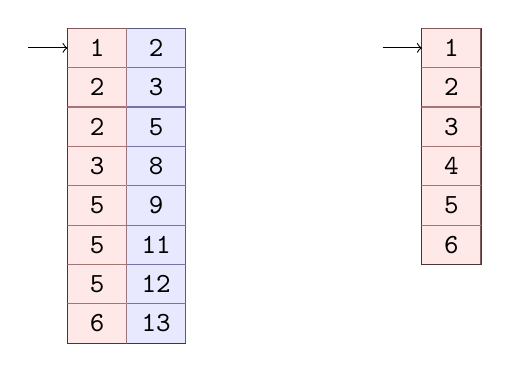
\begin{tikzpicture}
        \tuplesorted

        \draw[->] (-0.5, -0.25) -- (0, -0.25);
        \draw[->] (4, -0.25) -- (4.5, -0.25);
    \end{tikzpicture}
\end{figure}
\noindent Since the join query is based on a foreign key and a primary key, one of these blocks must have unique entries. In this case, it is the block on the left. We always go down the non-unique set of entries more frequently (if present) than the unique set of entries. At this point, there is a match between the two values in the blocks. We move down the non-unique block.
\begin{figure}[H]
    \centering
    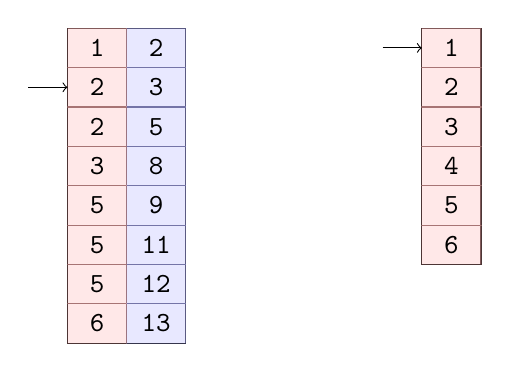
\begin{tikzpicture}
        \tuplesorted

        \draw[->] (-0.5, -0.75) -- (0, -0.75);
        \draw[->] (4, -0.25) -- (4.5, -0.25);
    \end{tikzpicture}
\end{figure}
\noindent There is a mismatch here- the entry \texttt{2} on the left is bigger than the entry \texttt{1}. So, we move down the right block as well.
\begin{figure}[H]
    \centering
    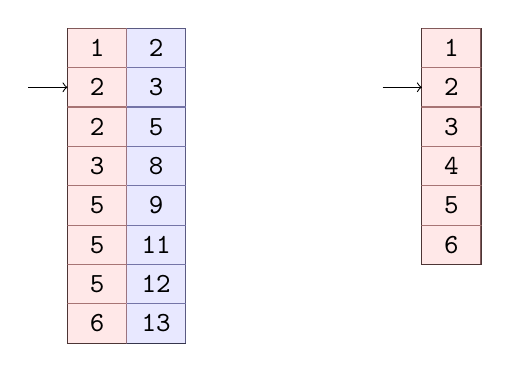
\begin{tikzpicture}
        \tuplesorted

        \draw[->] (-0.5, -0.75) -- (0, -0.75);
        \draw[->] (4, -0.75) -- (4.5, -0.75);
    \end{tikzpicture}
\end{figure}
\noindent There is a match in this case as well. We move down the non-unique block again.
\begin{figure}[H]
    \centering
    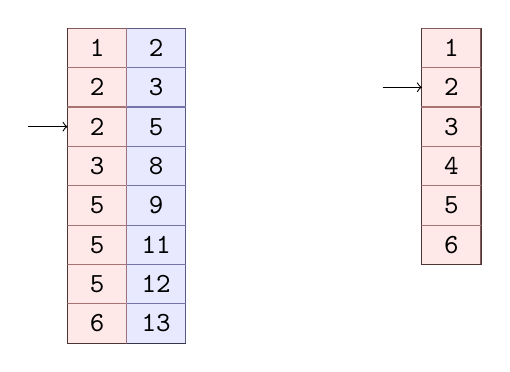
\begin{tikzpicture}
        \tuplesorted

        \draw[->] (-0.5, -1.25) -- (0, -1.25);
        \draw[->] (4, -0.75) -- (4.5, -0.75);
    \end{tikzpicture}
\end{figure}
\noindent There is another match in this case. We continue this process to join the two blocks.

\subsubsection{Hash join}
Now, if \texttt{R} and \texttt{S} are partioning into $M$ buckets with the same hash function over the join attributes \texttt{A} and \texttt{B}, then we can use a hash-join algorithm. Assuming \texttt{R} is the smallest file and fits into main memory, i.e. $M$ buckets of \texttt{R} are in memory, we start by partioning.
\begin{verbatim}
for each tuple r in R:
    compute y = h(r.A) // the address of the bucket
    place tuple r into bucket y = h(r.A) in memory
\end{verbatim}
Next, we have the probing phase.
\begin{verbatim}
for each tuple s in S:
    compute y = h(s.B) // using the same hash function
    find the bucket y = h(s.B) in memory
    for each tuple r in R in the bucket y:
        if s.B = r.A:
            add(r, s) to the result file;
\end{verbatim}
% TODO: Illustrate
In this case, we need to access each block precisely once. If \texttt{R} does not fit in memory, then we need $3(b_R + b_S)$ block accesses.

\newpage

\section{Selection selectivity}
There are two fundamental concepts in optimisation- join and selection selectivity. Selection selectivity is the fraction of tuples satisfying a condition. Join selectivity is the fraction of matching tuples in the Cartesian product.

Before running a query, we would like to predict the selection and the join selectivity, and hence the number of blocks we expect to retrieve. Then, using the actual block accesses, we aim to refine the expected cost. The expected cost is expressed as a function of selectivity. Using this result, we choose the optimal strategy to run a query.

In query optimisation, we are given a query as an input. The output is the optimal execution plan. There are two types of query optimisations:
\begin{itemize}
    \item Heuristic optimisation- we transform a SQL query into an equivalent and efficient query using Relational Algebra.
    \item Cost-based optimisation- we provide many execution plans and estimate their costs, and choose the plan with the minimum cost.
\end{itemize}
The cost function is what we want to optimise. It has parameters- the number of block accesses, the memory requirements, the CPU computational cost, the network bandwith, etc. We will consider the number of block accesses and memory requirements. 

We will use statistical information available to estimate the execution of a query. To do this, we store the following information for each relation:
\begin{itemize}
    \item the number of records $r$, and the (average) size of each record $R$.
    \item the number of blocks $b$, and the blocking factor $f$.
    \item the primary file organisation (heap, hash or sequential).
    \item the available indices- primary, clustering, secondary or B+ Trees.
\end{itemize}
For each attribute, we further store the following:
\begin{itemize}
    \item the number of distinct values (NDV) $n$ of the attribute.
    \item the domain range- the minimum and the maximum value of the attribute (among the tuples).
    \item the type of attribute- continuous or discrete, key or non-key.
    \item level $t$ of Index of the attribute, if present.
    \item the probability distribution function $P(A = x)$, which indicates the frequency of each value $x$ of the attribute $A$ in the relation.
\end{itemize}
A good approximation of the distribution is a histogram.

Selection selectivity of an attribute $A$, denoted by $\textit{sl}(A)$, is the fraction of tuples that satisfy a given condition. Therefore, its value is between 0 and 1. If $\textit{sl}(A) = 0$, then none of the records satisfy this condition with respect to the attribute $A$. On the other hand, if $\textit{sl}(A) = 1$, then all the records satisfy the condition with respect to the attribute $A$. As a probability, the selection selectivity tells us how likely is it for a tuple to satisfy the given condition with respect to an attribute.

The selection cardinality $s$ is the number of tuples we expect to satisfy a query with respect to a given attribute. In other words, the selection cardinality
\[s = \textit{sl}(A) \cdot r,\]
where $r$ is the number of tuples present. So, the value is between 0 and $r$. We predict this value without scanning any block. For example, if $r = 1000$ and $\textit{sl}(A) = 0.3$, then the selection cardinality $s = 300$. 

To predict selectivity, we can approximate the distribution of attribute values using a histogram. This allows us to maintain an accurate selectivity estimate. However, we must maintain this histogram whenever there is a change to the attribute for any of the tuples. In this case, we assume that
\[\textit{sl}(A = x) \approx P(A = x).\]
That is, the selection selectivity is approximately equal to the probability that the value of the attribute is that value.

Another possible approximation is that all values are uniformly distributed. This means that we do not need to maintain a histogram- all the values are of equal probability, so we barely need to store one value. However, we provide a less accurate prediction for the selection selectivity. In this case, we assume that
\[\textit{sl}(A = x) \approx \frac{1}{n},\]
where $n$ is the number of distinct values of $A$. Note that the selectivity is a constant value independent of $x$. 

If $A$ is a key attribute, then
\[\textit{sl}(A = x) \approx \frac{1}{r}\]
is a good estimate. There is only one tuple that satisfies the condition, so the selection cardinality $s = 1$. So, the uniformity assumption is valid in this case. We do not need to build a histogram.

Now, if $A$ is a non-key attribute, with $n = NDV(A)$, the number of distinct values of $A$ present. Then, the estimate
\[\textit{sl}(A = x) \approx \frac{1}{n}\]
is not a good estimate. This is under the assumption that all the records are uniformly distributed across the $n$ distinct values. This is not true in general.

Next, consider the following range selection selectivity.
\begin{lstlisting}[language=SQL]
SELECT  *
FROM    <relation>
WHERE   A >= x;
\end{lstlisting}
The domain range is defined to be $\max (A) - \min (A)$, and the query range in this case is $\max(A) - x$. If $x > \max(A)$, then $\textit{sl}(A \geq x) = 0$. Otherwise,
\[\textit{sl}(A \geq x) = \frac{\max(A) - x}{\max(A) - \min(A)},\]
under the uniformity assumption.

In particular, if we have $r = 1000$ employees, the attribute value ranges from $100$ to $10 \ 000$ and $x = 1000$, then the selection selectivity is
\[\textit{sl}(A \geq 1000) = \frac{\max(A) - x}{\max(A) - \min(A)} = \frac{10 \ 000 - 1000}{10 \ 000 - 100} = 0.909\]
In that case, the selection cardinality is $909$ tuples.

Now, consider the conjunctive selectivity, i.e. a query satisfying 2 conditions. An example is given below.
\begin{lstlisting}[language=SQL]
SELECT  *
FROM    <relation>
WHERE   (A = x) AND (B = y);
\end{lstlisting}
If the two attributes $A$ and $B$ are statistically independent, then the selectivity of the conjunction query $q$ is
\[\textit{sl}(q) = \textit{sl}(A = x) \cdot \textit{sl}(B = y).\]

Now, we consider a disjunctive selectivity condition, i.e. a query satisfying one of 2 conditions. An example is given below.
\begin{lstlisting}[language=SQL]
SELECT  *
FROM    <relation>
WHERE   (A = x) OR (B = y);
\end{lstlisting}
Then, the selection selectivity of this query is
\[\textit{sl}(Q) = \textit{sl}(A) + \textit{sl}(B) - \textit{sl}(A) \textit{sl}(B).\]
Here as well, we assume that the two attributes $A$ and $B$ are statistically independent.

Now, assume that we have $r$ tuples, and the attribute $A$ has $n$ number of distinct values. Under the uniform assumption of the attribute, the expected number of block accesses is
\[\operatorname{ceil}(s/f) = \operatorname{ceil}(r/f \cdot n),\]
where $s$ is the selection cardinality and $f$ is the blocking factor. The graph below summarises this.
% TODO: ADD GRAPH

Now, we apply this formula to refine the selection cost. Assume that we have the query
\begin{lstlisting}[language=SQL]
SELECT  *
FROM    <relation>
WHERE   A = x;
\end{lstlisting}
We have $b$ blocks; the blocking factor is $f$; we have $r$ records; and the number of distinct values of the attribute $A$ is $n$. We propose different approaches and the expected number of block accesses in each case.
\begin{itemize}
    \item Assuming that the tuples are sorted with respect to the attribute $A$, we can use a binary search algorithm. 
    \begin{itemize}
        \item If $A$ is a key attribute, then the expected cost is $\log_2 b$ block accesses. It is independent of the selection selectivity.
        \item If $A$ is not a key attibute, then it takes $\log_2 b$ block accesses to find the first block with record $A = x$. We then access all the contiguous blocks whose records satisfy $A = x$. This takes $\operatorname{ceil}(s/f) - 1$ further block accesses. In total, the expected cost is
        \[\log_2 b + \operatorname{ceil}(s/f) - 1 = \log_2 + \operatorname{ceil}(r \cdot \textit{sl}(A)/f) - 1.\]
        This is a function of the selection selectivity.
    \end{itemize}

    \item Now, assume that we have a level-$t$ multilevel primary/clustering index on the attribute.
    \begin{itemize}
        \item If $A$ is a key attribute, then the expected cost is $t + 1$ block accesses. It is independent of the selection selectivity.
        \item If $A$ is a non-key attribute, then it takes $t$ block accesses to descend the tree. The selection cardinality is $s = r \cdot \textit{sl}(A)$ tuples. So, we require $\operatorname{ceil}(s/f)$ block accesses, where $f$ is the blocking factor. So, the expected cost is
        \[t + \operatorname{ceil}(s/f) = t + \operatorname{ceil}(r \cdot \textit{sl}(A)/f).\]
        This is a function of the selection selectivity.
    \end{itemize}

    \item Assume next that we have a level-$t$ B+ tree on the attribute.
    \begin{itemize}
        \item If $A$ is a key attribute, then the expected cost is $t + 1$ block accesses. It is independent of the selection selectivity.
        \item If $A$ is a non-key attribute, then it takes $t$ block accesses to descend the tree. At this point, we have access to the block pointer to all the blocks containing a tuple satisfying the condition. The selection cardinality is $s = r \cdot \textit{sl}(A)$ tuples. Since the tuples are not sorted with respected to $A$, we assume that we must access $s$ blocks to retrieve all the tuples. In that case, the expected number of block accesses is
        \[t + 1 + s = t + 1 + r \cdot \textit{sl}(A).\]
        This is a function of the selection selectivity.
    \end{itemize}

    \item Finally, assume that we are using a hash file structure. For any attribute $A$, then the expected cost is just 1 block access (if there are no overflown buckets). This is independent of the selection selectivity.
\end{itemize}

Next, assume that we have the query
\begin{lstlisting}[language=SQL]
SELECT  *
FROM    <relation>
WHERE   A >= x;
\end{lstlisting}
\begin{itemize}
    \item Assume further that we have a level $t$ primary index and $A$ is a key attribute. We traverse the tree in $t$ block access, finding the data block for $A = x$. Then, the range selection cardinality is 
    \[s = r \cdot \textit{sl}(A \geq x).\]
    So, we further access $\operatorname{ceil}(s/f)$ blocks since the file is sorted with respect to this attribute. In total, we have
    \[t + \operatorname{ceil}(s/f) = t + \operatorname{ceil}(r \cdot \textit{sl}(A)/f)\]
    block accesses. This is a function of the selection selectivity.
    \item Now, assume that we have a level $t$ B+ tree and $A$ is a key, non-ordering attribute. We traverse the tree in $t$ block access, finding the data block for $A = x$. Then, the range selection cardinality is
    \[s = r \cdot \textit{sl}(A \geq x).\]
    Since the file is not sorted with respect to this attribute, we further access $s$ blocks in the worst case. In total, we have
    \[t + s = t + r \cdot \textit{sl}(A)\]
    block accesses.
\end{itemize}
\newpage

\section{Join selectivity}
We measure join selectivity with respect to the cartesian product of the two relations. For example, consider the following tables.
\begin{table}[H]
    \centering
    \begin{tabular}{|c|c|c|}
        \hline
        \texttt{SSN} & \texttt{Name} & \texttt{DNO} \\
        \hline
        1 & Chris & D1 \\
        2 & Stella & D1 \\
        3 & Phil & D2 \\
        4 & Thalia & D3 \\
        5 & John & D3 \\
        \hline
    \end{tabular}

    \hspace{10pt}

    \begin{tabular}{|c|c|c|}
        \hline
        \texttt{DNumber} & \texttt{MGR\_SSN} & \texttt{DName} \\
        \hline
        D1 & 1 & HR \\
        D2 & 3 & R\&D \\
        D3 & 4 & SPR \\
        \hline
    \end{tabular}
\end{table}
\noindent Their Cartesian product has $5 \cdot 3 = 15$ entries. However, the following is the joined table with respect to \texttt{DNO} and \texttt{DNumber}.
\begin{table}[H]
    \centering
    \begin{tabular}{|c|c|c|c|c|}
        \hline
        \texttt{SSN} & \texttt{Name} & \texttt{DNO} & \texttt{MGR\_SSN} & \texttt{DName} \\
        \hline
        1 & Chris & D1 & 1 & HR \\
        2 & Stella & D1 & 1 & HR \\
        3 & Phil & D2 & 3 & R\&D \\
        4 & Thalia & D3 & 4 & SPR \\
        5 & John & D3 & 4 & SPR \\
        \hline
    \end{tabular}
\end{table}
\noindent There are only 5 entries here, so the join cardinality is 5. Moreover, the join selectivity is $5/15 = 1/3$.

If we are joining two relations $R$ and $S$, then the join selectivity is given by
\[\textit{js} = |R \bowtie S|/|R \times S|.\]
It is a value between 0 and 1. Moreover, the join cardinality is given by
\[\textit{jc} = \textit{js} \cdot |R| |S|.\]

We can predict the join selectivity/cardinality using the join selectivity theorem. Given $n = \text{NDV}(A, R)$ and $m = \text{NDV}(B, S)$, then
\[\textit{js} = 1/\max(n, m).\]
This implies that 
\[\textit{jc} = |R| |S| / \max(n, m).\]

We illustrate the this with an example. Assume that we have a relation \texttt{E} of employees and \texttt{D} of dependents. An employee can have multiple dependents. Their common attribute is \texttt{SSN} of the employee. We have
\begin{itemize}
    \item $n$ = NDV(SSN, \texttt{E}) = 2000 and $|E| = 2000$;
    \item $m$ = NDV(SSN, \texttt{P}) = 3 and $|P| = 5$.
\end{itemize}
Therefore, the join selectivity is
\[1/\max(n, m) = 1/2000 = 0.0005.\]
This implies that there is a 0.05\% probability of getting a matching tuple from the cartesian space.

Now, assume we have relations $R$ and $S$ with $b_R$ and $b_S$ blocks. They can be joined using \texttt{R.A = S.B}. In memory, we have $n_B$ blocks, and there are $n$ distinct values of \texttt{R.A} and $m$ distinct values of \texttt{S.B}. The blocking factor is $f_{RS}$ matching tuples per block. The size of the maching tuple $(r, s)$ is the sum of the size of the tuple $r$ and $s$. We wrtie every full result block to disk. We expect the result to have
\[\textit{jc} = \textit{js} \cdot  |R| |S| = |R| |S| /\max(n, m).\]
So, the number of result blocks is
\[k = (\textit{js} \cdot |R| \cdot |S|)/f_{RS}.\]
When executing a join query, this is the number of block accesses corresponding to store the result back into memory. This can be used for further processing of the data when it doesn't fit in memory, for example.  

\end{document}
